\pagebreak
\section{Implementazione del file system}
In questo capitolo ci occuperemo di discutere in dettaglio il modo in cui viene implementato il file system. Capiremo che cos'è la struttura di un file systems e che tipo di operazioni supporta. Discuteremo inoltre come sono implementate le directories e i diversi metodi di allocazione del file systems: questi aspetti sono già stati citati nel capitolo precedente ma in questo capitolo scaviamo più nel profondo e cerchiamo di capire come questi siano effettivamente creati. Parleremo infine della gestione dello spazio libero e di performance. 

\subsection{Struttura e operazioni del file system}
La periferica fisica, come il disco, ci permette di leggere e scrivere i dati. Tipicamente è composto di \textbf{blocchi} che vanno da 512 a 49 bytes. Il file system risiede sulla memoria secondaria e che fornisce l'interfaccia utente per memorizzare tali dati mappando il loro indirizzo logico in un indirizzo fisico sul disco. Inoltre il file system deve anche essere in grado di fornire lo spazio sulla feriferica in modo efficiente. 
% 
\subsubsection{Livelli}\label{layers}
\begin{wrapfigure}{o}{.30\textwidth}
  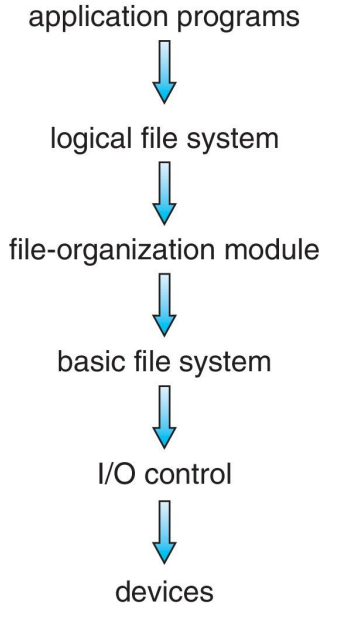
\includegraphics[width = \linewidth]{../res/imgs/file system implementation/file system layers.png}
  \caption{I livelli del file system.}
  \label{fig:file system layers}
\end{wrapfigure}
Il file system non è un singolo blocco ma lo si può considerare come un struttura organizzata a diversi livelli. Osserviamo la figura \ref{fig:file system layers} e discutiamo i diversi livelli.
Il \textbf{controllo I/O} viene effettuato attraverso i \textit{device-drivers} (già discussi nel paragrafo \ref{device-drivers}) e attraverso gli \textit{interrupt handlers} (vedi paragrafo \ref{interrupt handler}). Questo si occupa di tradurre comandi del tipo \texttt{read drive3, cylinder 14, traccia 15, settore 92} nella locazione di memoria \texttt{6535}. Salendo di un livello incontriamo il \textbf{basic file system} che gestisce comandi del tipo \texttt{read block 12} di un determinato indirizzo logico. Questo gestisce anche eventuali buffer che possono essere eventualmente utilizzati per la trasmissione della periferica alla memoria e di cache, utili per mantenere una copia dei blocchi utilizzati più frequentemente. Dopo di che troviamo il \textbf{modulo di organizzazione dei file} che è in grado di interpretare la struttura dei file e il loro indirizzo logico. Si occupa di tradurre l'indirizzo logico in indirizzo fisico e gestisce il \textit{free space} (vedi \ref{free space}). Infine, poco più sotto del livello di applicazione, troviamo il \textbf{logical file system} che si occupa di gestire i \textit{metadata} e strutture di alto livello. Per esempio è responabile della traduzione dei nomi dei file in un ID, identificativo numerico che viene utilizzato dai livelli sottostano. Mantiene inoltre il \textit{file control block} (\ref{FCB}), chiamato anche \textbf{inode} in UNIX. Oltre a ciò gestisce anche la struttura delle directory (discusse nel paragrafo \ref{directory}) e la protezione (paragrafo \ref{protection}).

Questa stratificazione del file system è stata ideata per ridurre la complessità di tutte le operazioni da effettuare però ha lo svantaggio perché introduce un \textbf{overhead} che in alcuni casi può decrementare l'effettiva performance. Ecco perché in alcuni applicativi non è presente uno specifico file system per memorizzare dati per evitare di andare attraverso questi layers. Queste operazioni sono infatti lasciate all'effettivo \textit{database} che gestisce i dati.

% 
\subsubsection*{Tipi}
Possiamo trovare una grande vastità di file systems implementati in maniera divers. Alcuni di questi sono dedicati a perficeriche removibili come nel caso della ISO 9660, utilizzata per i CD. Altri invece variano a seconda del sistema operativo dato che sistemi operativi diversi spesso sono pensati per operazioni diverse. Ecco quindi che in Unix troviamo \textbf{UFS}, in Windows, storicamente FAT (\ref{FAT}), e adesso \textbf{NTFS} mentre in Linux troviamo \textbf{ext3} ed \textbf{ext4}. Citiamo anche il \textbf{ZFS}, trovato in Solaris e GoogleFS che sono più recenti.

% 
\subsubsection{Strutture per le operazioni}
Naturalmente il file system deve supportare operazioni per lavorare con i dati. Per fare ciò necessita di contenere delle strutture dati per agevolare e implementare tali operazioni. Possiamo dividere le strutture in due tipo: quelle che risiedono sul disco e quelle che vivono in memoria. 

Sul disco troviamo tipicamente dei blocchi dedicati al booting ovvero i \textbf{boot control block} che servono appunto fare partire il sistema operativo: fare eseguire il minimo necessario per poi far partire il kernel e tutto il resto. È inoltre presente il \textbf{volume control block} che contiene informazioni sul volume: il numero totale di blocchi sul device oppure il numero di blocchi liberi. Infine è presente la \textbf{directory} - o almeno parte di essa - che, come sappiamo (\ref{directory}), è utilizzata per organizzare i files: contiene quindi anche gli FCB.

Nella memoria invece sono presenti le strutture per implementare le system calls. Troviamo quinti la \textbf{mount table}, che contene le parti che sono collegate al sistema operativo. È presente anche la \textbf{in-memory directory structure}, ovvero la memoria che si occupa detenere le informazioni riguardanti le directory utilizzate più recentemente. Nella memoria possiamo anche trovare \textbf{system-wide open-file table} ovvero la tabella di sistema dei file aperti che contiene una copia degli FCB (\ref{FCB}). Come c'è la tabella di sistema è presenta anche una tabella con i FCB dei files aperti per ogni processo. Infine sono anche presenti dei buffers per agevolare le operazioni di lettura e scrittura.

% 
\subsubsection{File Control Block (FCB)}\label{FCB}
Il \textit{File Control Block}, già menzionato molte volte all'interno di questo capitolo, è una struttura mantenuta dal sistema operativo che, per ogni file, contiene diverse informazioni riguardanti tale file. Dalla figura \ref{fig:FCB} possiamo notare che in genere sono memorizzati i permessi del file (come le liste di accesso, \ref{permissions}),
\begin{figure}[h]
    \centering
    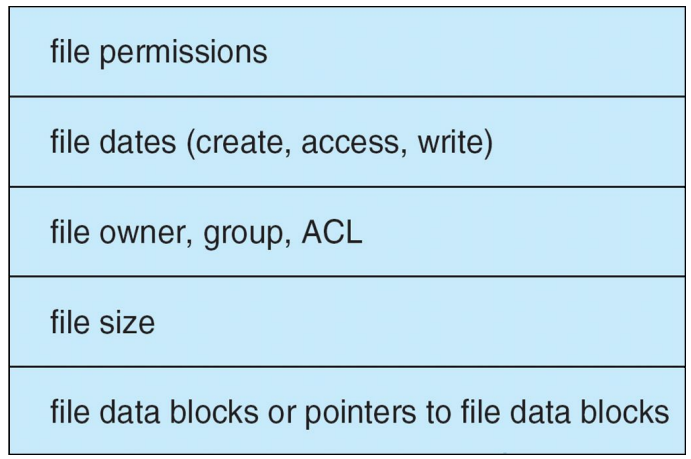
\includegraphics[width = .45\textwidth]{../res/imgs/file system implementation/FCB.png}
    \caption{La struttura del \textit{File Control Block}}
    \label{fig:FCB}
\end{figure}
informazioni temporali (come la creazione o l'ultimo accesso), proprietà, dimensione e altre informazioni rigaurdanti il reperimento di informazioni del file come puntatori. 
\todo{completa slide 10 e 11 (minuto 18 - 24}

% 
\subsection{Metodi di allocazione}
Arriviamo al punto più critico: come avviene effettivamente allocato lo spazio sul disco per contenere i file? Ci sono tre tecniche principali - allocazione contigua, concatenata e indicizzata - e le approfondiremo tutte in questo paragrafo.

\subsubsection{Allocazione contigua}
Nell'allocazione contigua il disco viene diviso in un numero di blocchi che possono essere da 512 byte o 4096 byte. I file sono quindi allocati in \textbf{locazione contigue}, una vicina all'altra.
\begin{figure}[h]
    \centering
    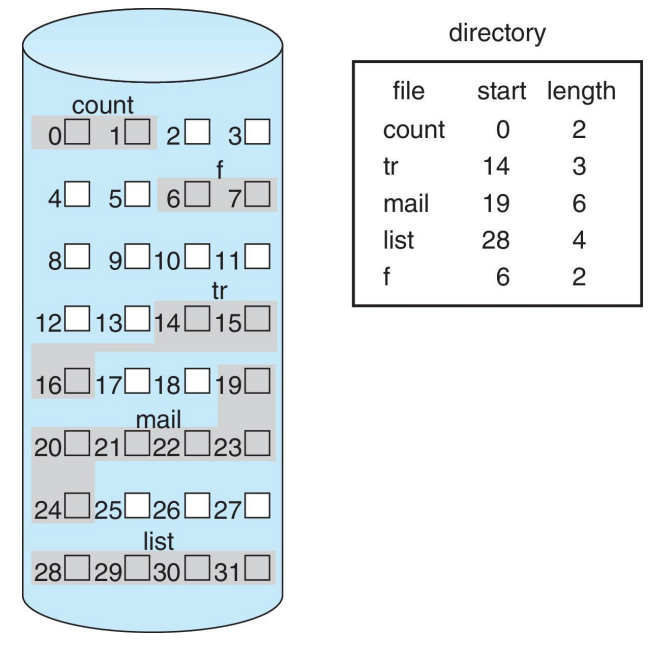
\includegraphics[width = .55\textwidth]{../res/imgs/file system implementation/allocazione contigua.png}
    \caption{Rappresentazione dell'allocazione contigua su disco.}
    \label{fig:allocazione contigua}
\end{figure}
Ricordiamo che sia nel caso di dischi elettromeccanici ma anche negli SSD blocchi vicino corrispondono ad una velocità maggiore in accesso. Osservando l'illustrazione \ref{fig:allocazione contigua} possiamo notare che non è nemmeno difficile da implementare: è necessario solamente memorizzare la locazione del blocco iniziale e la dimensione/lunghezza del file: per esempio il file \texttt{mall} parte dalla locazione 19 e ne occupa 6; possiamo infatti notare che i blocchi, dal 19 al 24, sono ingrigiti in quanto occupati.

Questa soluzione però porta con sé dei problemi non indifferenti. Innanzitutto è necessario conoscere la lunghezza del file, ma non è sempre possibile saperlo, soprattutto se si tratta di un file che magari viene modificato (per esempio un documento). Ancora più grave è la \textbf{frammentazione esterna}: questo significa che all'interno del disco è presente dello spazio ma questo spazio non è contiguo. Per esempio, sempre facendo riferimento alla figura \ref{fig:allocazione contigua}, se dovessimo inserire un file di lunghezza 7 questo non sarebbe possibile anche se sono presenti più di 7 blocchi liberi nel disco. Si possono adottare delle tecniche per fare una \textbf{compattazione} dove, per esempio, si trasferiscono tutti i file in un altro \textit{storage} per poi ricopiarli uno dopo l'altro in modo tale da renderli tutti attaccati. Questa però rimane una soluzione non ottimale in quanto nel caso di grandi \textit{data centers} non è possibile bloccare il sistema per fare questi trasferimenti.

Un possibile miglioramento di questa tecnica si basa sull'uso di \textbf{extent}, non a caso questa versione migliorata è chiamata \textit{extent-based system}. Un extent è un insieme di più blocchi contigui sul disco. Possiamo dire che è un approccio semi-contiguo nel senso che è contiguo sicuramente per tutta la lunghezza di un extent. Questa soluzione è implementata nel \textit{Veritas file system}. 

% 
\subsubsection{Allocazione concatenata}
In questa tecnica, al posto di utilizzare una disposizione contigua si sceglie di disporre il file in una lista di blocchi non contigui i quali possono essere sparsi all'interno del disco. Come possiamo osservare dalla figura \ref{fig:allocazione concatenata} questo comporta la necessità di avere un puntatore in un blocco $n$ che punta al blocco $n + 1$.
\begin{figure}[h]
    \centering
    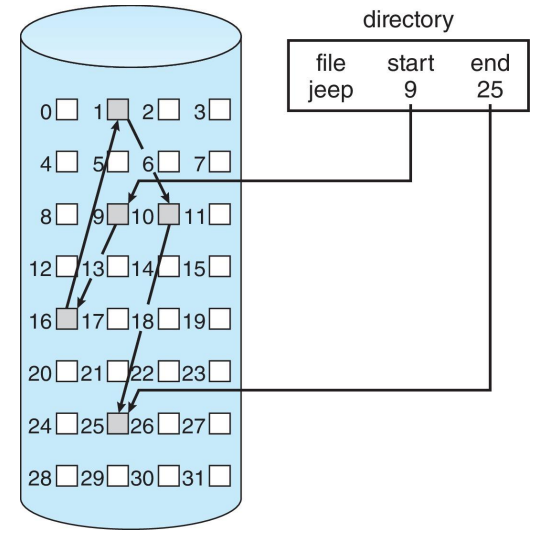
\includegraphics[width = .5\textwidth]{../res/imgs/file system implementation/allocazione concatenata.png}
    \caption{Rappresentazione dell'allocazione concatenata.}
    \label{fig:allocazione concatenata}
\end{figure}
Di conseguenza, all'interno di ogni blocco, è necessario utilizzare dello spazio per memorizzare il puntatore al blocco successivo. Per esempio, se i blocchi occupano 512 bytes e il sistema dispone di indirizzi a 4 bytes (32 bit) allora in ogni blocco si possono memorizzare $512 - 4 = 508$ bytes di file. Non è un valore eccessivamente grande ($\frac{1}{100}$) ma è bene tenerne conto.

Il vantaggio è che la frammentazione esterna presente nell'allocazione contigua non è più un problema. D'altro canto però non è un'ottima tecnica se si vuole avere un accesso \textbf{random} in quanto al fine di arrivare al blocco $n$ si devono effettuare $n - 1$ accessi in lettura dato che è necessario scorrere tutta la lista. Per migliorare l'accesso diretto si può \textit{clusterizzare} i blocchi: al posto di avere dei blocchi isolati si possono avere dei gruppi di blocchi contigui cosicché da scorrerli una volta raggiunti. Questa soluzione però aumenta la \textbf{frammentazione interna} nel caso in cui lo spazio allocato da quel \textit{cluster} non venga utilizzato completamente. Infine, l'ultimo problema di questa soluzione si ha nel caso in cui un \textbf{blocco} sia \textbf{corrotto} (a livello di bug oppure anche fisicamente). Questo perché non sarebbe più possibile raggiungere la parte della lista seguente al blocco.

Un esempio di questo tipo di allocazione è la storica \textbf{FAT} (\textit{File-Allocation Table}, figura \ref{fig:FAT})\label{FAT} che era un tempo utilizza nei sistemi MS-DOS e si trova tutt'ora in qualche applicazione
\begin{figure}[h]
    \centering
    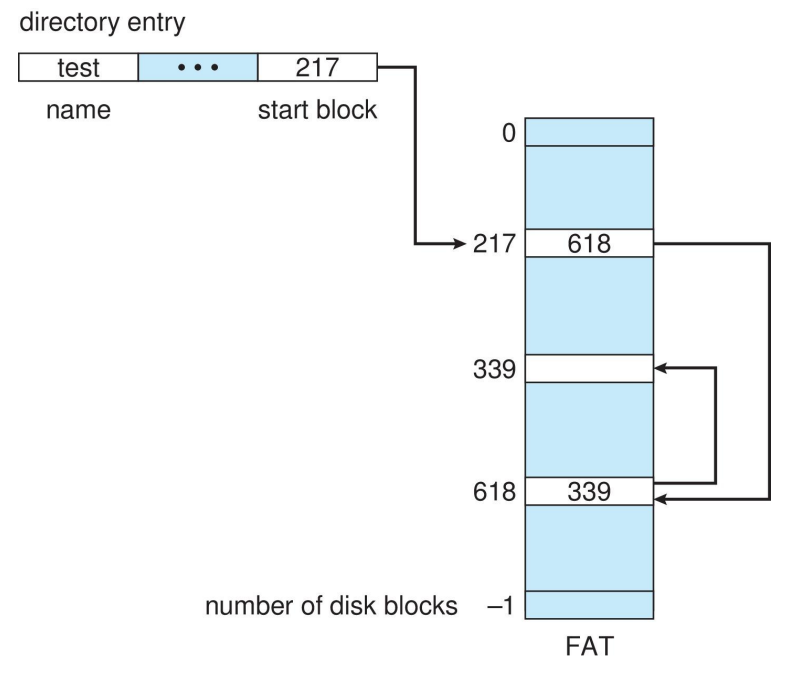
\includegraphics[width = .55\textwidth]{../res/imgs/file system implementation/FAT.png}
    \caption{La tabella FAT.}
    \label{fig:FAT}
\end{figure}
Questa è una tabella dedicata che è detenuta all'inizio del volume del disco ed ogni elemento di tale tabella contiene l'indice del blocco successivo. Quindi per identificare quali sono i blocchi di un determinato file è sufficiente mantenere l'informazione nella directory del blocco iniziale e poi nella \textit{file table} c'è la posizione dell'elemento successivo e così via fino a che non si raggiunga la fine del file. Con questa strategia, per effettuare l'accesso su un file non è necessario scorrere gli effettivi blocchi sul file bensì è sufficiente scorrere la FAT che rappresenta la struttura di quei blocchi. 

% 
\subsubsection{Allocazione indicizzata}
L'ultimo metodo che abbiamo elencato è il metodo di allocazione indicizzata. Anche questa tecnica si basa sui puntatori ma cerca di utilizzarli in maniera efficiente. Come è possibile notare nell'illustrazione \ref{fig:allocazione indicizzata}, al posto di salvare su ogni blocco un puntatore (o indirizzo) al blocco successivo, è più efficiente memorizzare tutti gli indirizzi tutti i blocchi del file su un unico blocco, chiamato \textbf{index block}.
\begin{figure}[h]
    \centering
    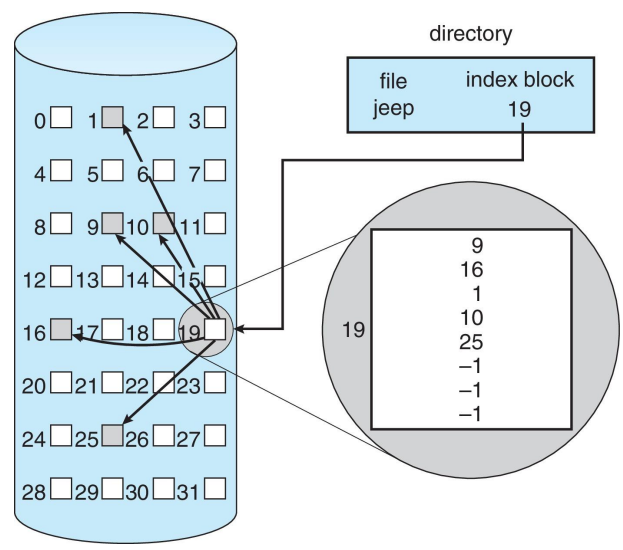
\includegraphics[width = .6\textwidth]{../res/imgs/file system implementation/allocazione indicizzata.png}
    \caption{Rappresentazione dell'allocazione indicizzata.}
    \label{fig:allocazione indicizzata}
\end{figure}
Così facendo, con $n$ blocchi, $n - 1$ blocchi sono utilizzati per la pura memorizzazione mentre l'ultimo è utilizzato per collegarli tutti. Dunque non si ha più una struttura sequenziale come nell'allocazione concatenata ma si ha una strutta simile a quella di una ragnatela. Per files molto grandi, inoltre, è possibile utilizzare uno blocco fra gli $n - 1$ restanti e utilizzarlo anch'esso per indicizzare altri $m - 1$ blocchi.

In questo caso il problema è che se il file è molto piccolo, gran parte dell'index block è sprecato: si incombe quindi nella frammentazione interna. Ridurre la dimensione dei blocchi per evitare la frammentazione interna non è una buona idea perché elimina il problema ma nel caso di files di grandi dimensioni si necessitano molti più index blocks. Ecco quindi che si è scelto di migliorare questa tecnica attraverso diverse versioni. Nello \textbf{schema concatenato} si utilizzano dei blocchi di piccole dimensioni andando quindi a creare più blocchi indice collegati tra loro (strutturalmente diventa una sequenza di piccole ragnatele). Nello schema con \textbf{indice multi-livello} il blocco indice di primo livello contiene gli indirizzi a blocchi indice di secondo livello aumentando notevolmente lo spazio di indirizzamento.

Infine c'è lo \textbf{schema combinato} che mescola le versioni precedenti ed è quello che tuttora viene utilizzato in Unix e Linux dove abbiamo a che fare con l'\textbf{inode} che, come visto in \ref{layers}, non è altro che il \textit{File Control Block} di Linux.
\begin{figure}[h]
    \centering
    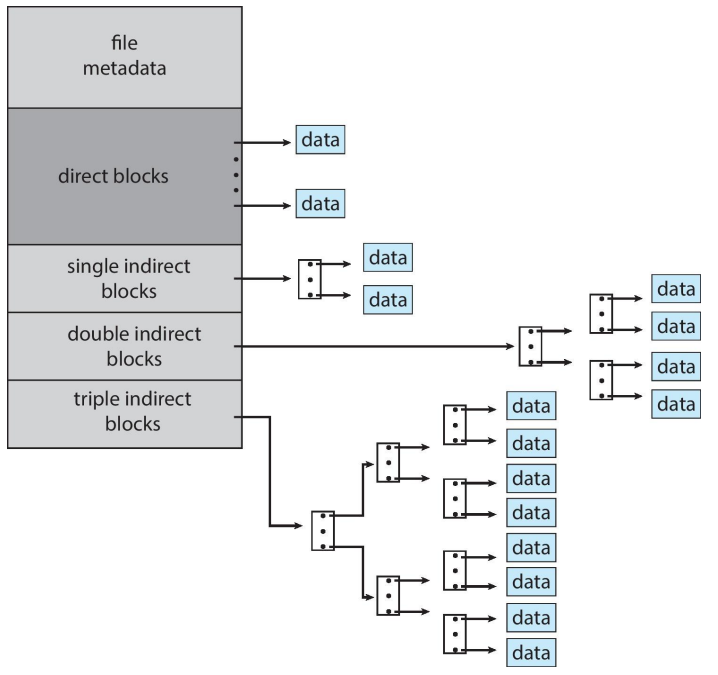
\includegraphics[width = .6\textwidth]{../res/imgs/file system implementation/schema combinato.png}
    \caption{Rappresentazione dell'allocazione indicizzata - schema combinato.}
    \label{fig:schema combinato}
\end{figure}
Osservando la figura \ref{fig:schema combinato}, osserviamo che all'interno dell'inode sono presenti 15 puntatori:
\vspace{-5px}
\begin{itemize}
\setlength{\itemsep}{-.15 em}
    \item I primi 12 puntatori fanno riferimento diretto ai \textit{datablock} che si trovano sul disco, si chiamano infatti \textbf{direct blocks}. Di conseguenza se dobbiamo accedere ad un file con dimensione minore di 12 blocchi è possibili utilizzare questi puntatori;
    \item Il 13esimo puntatore è usato come \textbf{single indircet block}; ciò significa che contiene un puntatore ad un blocco puntatori. Di conseguenza per accedere ai dati è necessario accedere ai blocchi puntatore (che si trovano sul disco) e da lì essere indirzzato al dato effettivo (si fanno quindi 3 "salti", uno per il promo blocco, uno per il secondo e uno per leggere il dato);
    \item Il 14esimo e il 15esimo rappresentano il \textbf{double} e \textbf{triple} \textit{indirect block} che hanno due e tre livelli di blocchi puntatore (che si trovano tutti sul disco).
\end{itemize}
Supponiamo che un blocco sia di 512 byte e gli indirizzi siano a 32 bit (4 byte), con il \textit{single indirect block} possiamo indirizzare $\frac{512}{4}\cdot512 = 128\cdot512$ bytes (64KB), con il \textit{double} $128^2\cdot512$ bytes (8MB) e con il \textit{triple} $128^3\cdot512$ bytes (1GB).

Il vantaggio di questo schema è che la complessità arriva solo nel caso in cui si lavora con file di grandi dimensioni. Se invece si lavora sempre con file sufficientemente piccoli (6KB) si avranno a disposizioni i 12 puntatori iniziali che sono molto più rapidi rispetto agli ultimi 3. Si nota infatti che l'inode risiede nella memoria e di conseguenza per effettuare l'accesso ai blocchi puntati dai 12 puntatori l'unica accesso al disco che si effettua è proprio quello di prelevamento del file. 

% 
\subsubsection{Performance}\label{performance SSD}
Come abbiamo notato è che il metodo migliore in assoluto non esiste ma è strettamente legato al tipo di accesso che effettuiamo. Se infatti l'accesso è sequenziale quasi tutte le tecniche vanno più che bene. Se invece l'accesso è di tipo random la scelta della tecnica gioca una ruolo significativo. Inoltre è importante aver chiaro che non è assolutamente detto che le tecniche più complesse siano le migliori: se prendiamo in considerazione un sistema di backup che memorizza dei file enormi (GB oppure TB) in modo contiguo, non è assolutamente necessario implementare una struttura indicizzata come l'inode, è sufficiente utilizzare l'allocazione contigua che è molto più semplice da implementare.

È bene inoltre puntualizzare che nel caso delle memorie non volatili (paragrafo \ref{NVM}) come le SSD, le tecniche che abbiamo appena elencato non sono compatibili dato che le SSD sono fisicamente organizzate in maniera diversa rispetto agli HDD.

% 
\subsection{Gestione dello spazio libero}\label{free space}
Oltre alla memorizzazione dei dati, nella memoria secondaria è importante tenere traccia dei blocchi che sono liberi e utilizzabili in futuro. Tipicamente il sistema operativo mantiene la \textbf{free space list} che è una lista che tiene traccia dei blocchi (o cluster di blocchi) che sono liberi. Ci sono diversi metodi per implementare questa lista - come la free list o il grouping - e in questo paragrafo li discuteremo brevemente. 

Sprechiamo prima due parole sull soluzione più banale: il \textbf{bit vector} o, in alternativa, la \textit{bitmap}. Questa è una sequenza di $n$ bit che rappresentano gli $n$ blocchi; se il bit \textit{i}-esmo è impostato ad 1 significa che il blocco \textit{i}-esimo è libero. Per esempio sei sono liberi i blocchi 1, 3, 4, 5, 9 allora il bit vector sarà \texttt{101110001}.

% 
\subsubsection{Free list}
\begin{wrapfigure}{R}{.30\textwidth}
    \centering
    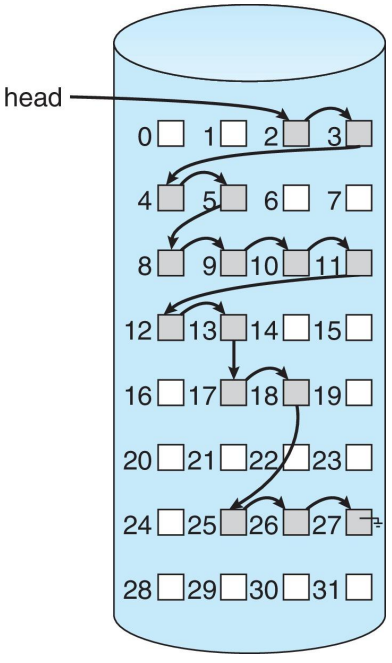
\includegraphics[width = .25\textwidth]{../res/imgs/file system implementation/free-space list.png}
\end{wrapfigure}
Ritornano anche in questo caso utili le liste. La free list è una lista che tiene traccia di tutti i blocchi che sono liberi all'interno del disco. Ciascun blocco in realtà non è completamente vuoto ma contiene, naturalmente, il puntatore al blocco libero successivo. Quindi l'unica cosa di cui dobbiamo tener traccia è il puntatore al primo blocco (\textbf{head}), a differenza invece della bitmap che cresce al crescere dello spazio di memorizzazione. Nel momento in cui si ha bisogno di un blocco si va ad occupare il primo e si aggiorna l'head al secondo blocco (che diventa quindi il primo). Ne consegue che, se abbiamo bisogno del primo blocco o dei primi $n$ blocchi, non è assolutamente necessario scorrerla tutta, quindi il problema della complessità non è così significativo. Inoltre non è facile ottenere dello spazio contiguo in quanto questo tipo di implementazione si occupa, ovviamente, di blocchi sparpagliati. 

% 
\subsubsection{Counting e grouping}\label{Counting}
\begin{wrapfigure}{L}{.3\textwidth}
    \centering
    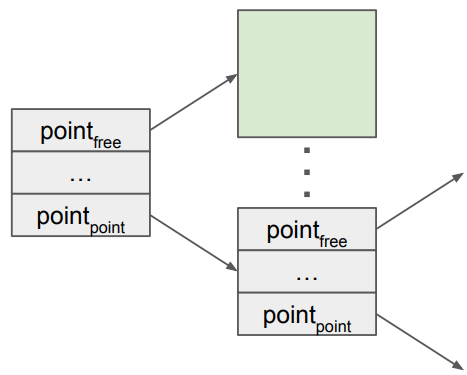
\includegraphics[width = .3\textwidth]{../res/imgs/file system implementation/grouping.png}
\end{wrapfigure}
Altre soluzioni lecite si ottengono attraverso un raggruppamento dei blocchi, come nel \textbf{grouping} (figura a lato): molto simile alla soluzione di indicizzazione multi-livello che abbiamo discusso precedentemente. Potremmo infatti avere un blocco dedicato che contiene tutti i blocchi liberi i quali, a loro volta, possono puntare a blocchi liberi. Il metodo \textbf{counting} invece, dato che spesso lo spazio è liberato in modo contiguo quindi è sufficiente tenere traccia del numero di blocchi successivi che sono liberi. Non è quindi sufficiente tenere traccia di un indirizzo e il numero di blocchi che, oltre a quell'indirizzo, sono liberi uno dopo l'altro. Nel caso in cui il contatore del numero di blocchi contigui è $> 1$ allora possiamo dire che l'implementazione di un contatore risulta più conveniente rispetto alla \textit{free list}.

% 
\subsubsection{Altri metodi}
Concludiamo menzionando altri metodi usati in altri file system che si occupano di risolvere altri problemi. Per esempio \textbf{ZFS} - presente in Solaris - divide lo spazio del disco in \textit{metaslab} i quali hanno associato una \textbf{spacemap} che è un log per memorizzare le attività effettuate in quella particolare zona del disco. Osserviamo inoltre che questo file system è ottimo per la gestione di files di grandi dimensioni grazie anche ad un algoritmo basato sul counting (\ref{Counting})

Menzioniamo anche un'altra tecnica, chiamata \textbf{TRIM}, che è un nuovo meccanismo utilizzato per gestire le NVM. Ricordiamo infatti che sulle SSD non è possibile effettuare un'operazione di sovrascrittura (vedi \ref{NVM}) bensì è necessario prima cancellare il blocco per poi scrivere la nuova informazione e quindi è necessario utilizzare delle strategia diverse. In questo caso il metodo TRIM riesce a ridurre la necessità di fare frequentemente \textit{garbage collection} e minimizza la possibilità di eliminare grandi blocchi di dati
